\documentclass{article}
\usepackage{graphicx}
\usepackage{hyperref}

\title{Derivation of a $\zeta,\lambda,c$ formulation of IRT}
\author{David N. Mashburn \\
        Pluralsight, LLC}
\date{2016-9-7}
\begin{document}
\maketitle

\section{Introduction}

Item Response Theory (IRT) is a field of study concerning the measurement
of ability based on item characteristic curves (ICC). ICC's have an upper and lower
horizontal asymptote and are described by a logistic function (or a normal ogive,
having nearly the same curve in practice). The ICC describes the
probability that a person with a given inherent ability (or latent trait)
will successfully answer an item (question). For more complete information
about IRT, see
\url{http://www.wikipedia.org/wiki/Item_response_theory}
and the book "Item Response Theory: Parameter Estimation Techniques" by
Frank B. Baker and Seock-Ho Kim
\url{http://www.crcpress.com/product/isbn/9780824758257}
\\
The notation below is all based on the treatment in Baker.
\\
\begin{center}
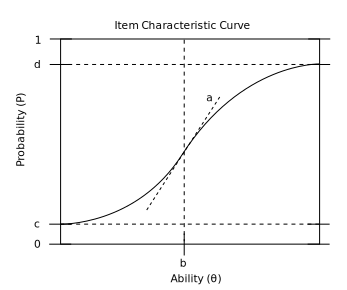
\includegraphics{item-characteristic-curve.pdf}
\end{center}

The features of the ICC are:

\begin{itemize}
  \item Item Difficulty (b) The point at which persons with that ability level
        or higher will score in the top 50th percentile on the item.
  \item Discriminatory Power (a) The ability of the question to split the
        population accurately. In the ideal case, the ICC becomes a step function.
  \item Pseudo-guessing Parameter (c) The probability that low-ability people
        can get the item correct.
  \item Upper Asymptote (d, rarely used) The probability that high-ability people
        can get the item correct (usually 1 or very nearly 1).
\end{itemize}

Together, these make up the 4 parameter logistic (4PL) model ($a,b,c,d$).
The more common 3PL includes only ($a,b,c$).
\\\\
The logistic function has this basic form:
\\\\
$P^*(\theta _j) = \frac{1}{e^{-f(\theta _j)}+1}$
\\\\
Where $f(\theta _j)$ is the logistic exponent (logit).
\\\\
Item Response Theory has two main mathematical bases:
the ($\lambda,\zeta$) formulation used in the 2 parameter logistic model (2PL)
and the ($a,b,c$) formulation used in the 3 parameter (3PL) model.
The logit in either case is:
\\\\
$\zeta +\lambda \theta _j = a \left(\theta _j-b\right)$
\\\\
Using this equivalence, we can easily see the relationships between ($a,b$) and ($\zeta, \lambda$)
\\\\
$a = \lambda$
\\\\
$\zeta = -a b$
\\\\
$b = -\frac{\zeta }{\lambda }$
\\\\
The rest of this document is devoted to deriving the following equations
for the novel ($\zeta,\lambda,c$) formulation of the logistic function:

\begin{itemize}
  \item Likelihood Function
  \item Jacobian of the Likelihood Function (1st derivatives)
  \item Hessian of the Likelihood Function (2nd derivatives)
\end{itemize}

These equations form the basis for the maximum likelihood estimation (MLE)
routines in this Python package.
The derivations will follow the same steps as in Chapter 2, section 2.6 of Baker,
but substituting for ($a,b$) using ($\lambda,-\frac{\zeta}{\lambda}$).
\\\\
\section{Derivations}
\subsection{Preliminaries}

$\Psi (Z_j)=(P_j){}^*=P^*(\theta _j)=\frac{1}{e^{-(\zeta +\lambda \theta _j)}+1}$
\\\\
$P_j=(1-c) \Psi (Z_j)+c$
\\\\
$P_j-c=(1-c) (P_j){}^*$
\\\\
$\Psi _j=(P_j){}^*=\frac{P_j-c}{1-c}$
\\\\
$Q_j=(1-c) (1-\Psi (Z_j))$
\\\\
$P_j=1-Q_j$
\\\\
$W_j=\frac{(P_j){}^* (Q_j){}^*}{P_j Q_j}$
\\\\
$p_j$ is the proportion correct
\\\\
$r_j = f_j p_j$
\\\\
\subsection{Generic Likelihood and Derivatives}

$L=\log (Prob(R))=(f-r) \sum \log (Q)+r \sum \log (P)+const$
\\\\
$\frac{\partial L}{\partial x}=r \sum \frac{1}{P}\frac{\partial P}{\partial x}+(f-r)\sum \frac{1}{Q}\frac{\partial Q}{\partial x}$
\\\\
$\frac{\partial L}{\partial x}=r \sum \frac{1}{P}\frac{\partial P}{\partial x}-(f-r)\sum \frac{1}{Q}\frac{\partial P}{\partial x}$
\\\\
$\frac{\partial L}{\partial x}=\sum (\frac{r}{P}-\frac{f-r}{Q})\frac{\partial P}{\partial x}$
\\\\
$\frac{\partial L}{\partial x}=\sum (\frac{Q r-P f+P r}{P Q})\frac{\partial P}{\partial x}$
\\\\
$\frac{\partial L}{\partial x}=\sum (\frac{ r-f P}{P Q})\frac{\partial P}{\partial x}$
\\\\
\subsection{Generic Logistic Function and Derivatives}

$\Psi (x)=\frac{1}{e^{-g(x)}+1}$
\\\\
$e^{-g(x)}=\frac{1}{\Psi }-1$
\\\\
$g=\zeta +\lambda \theta \frac{\partial g}{\partial \lambda }=\theta \frac{\partial g}{\partial \zeta }=1$
\\\\
with x either $\lambda$ or $\zeta$ :
\\\\
$\frac{\partial \psi }{\partial x}=\frac{e^{-g(x)} g'(x)}{(1+e^{-g(x)})^2}=\Psi ^2e^{-g(x)} \frac{\partial g}{\partial x}=\Psi ^2(\frac{1}{\Psi }-1)\frac{\partial g}{\partial x}=\psi (1-\Psi )\frac{\partial g}{\partial x}$
\\\\
\subsubsection{Partial Derivatives of P}

with x either $\lambda$ or $\zeta$ :
\\\\
$\frac{\partial P}{\partial x}=(1-c)\frac{\partial \Psi }{\partial x}$
\\\\
$\frac{\partial P}{\partial \lambda }=(1-c)\frac{\partial \Psi }{\partial \lambda }=(1-c)(1-\Psi )\psi \theta$
\\\\
$\frac{\partial P}{\partial \zeta }=(1-c)(1-\Psi )\psi$
\\\\
$(1-c)(1-\Psi )=(1-c)(1-\frac{P_j-c}{1-c})=1-c-P_j+c=1-P_j=Q$
\\\\
$\frac{\partial P}{\partial \lambda }=Q \psi \theta$
\\\\
$\frac{\partial P}{\partial \zeta }=Q \psi$
\\\\
$\frac{\partial P}{\partial c}=\frac{\partial }{\partial c}(c+(1-c)\Psi )=1-\psi =\frac{Q}{1-c}$
\\\\\
\subsection{Partial Derivatives of L}

$\frac{\partial L}{\partial x}=\sum (\frac{ r-f P}{P Q})\frac{\partial P}{\partial x}$
\\\\
$\frac{\partial L}{\partial \lambda }=\sum (\frac{ r-f P}{P Q})\frac{\partial P}{\partial \lambda }$
\\\\
$\frac{\partial L}{\partial \lambda }=\sum (\frac{ r-f P}{P Q})Q \psi \theta$
\\\\
$\frac{\partial L}{\partial \lambda }=\sum ( r-f P)\frac{\psi }{P} \theta$
\\\\
$\frac{\partial L}{\partial \zeta }=\sum (\frac{ r-f P}{P Q})\frac{\partial P}{\partial \zeta }$
\\\\
$\frac{\partial L}{\partial \zeta }=\sum (\frac{ r-f P}{P Q})Q \psi$
\\\\
$\frac{\partial L}{\partial \zeta }=\sum ( r-f P)\frac{\psi }{P}$
\\\\
$\frac{\partial L}{\partial c}=\sum (\frac{ r-f P}{P Q})\frac{\partial P}{\partial c}$
\\\\
$\frac{\partial L}{\partial c}=\sum (\frac{ r-f P}{P Q})\frac{Q}{1-c}$
\\\\
$\frac{\partial L}{\partial c}=\sum \frac{ r-f P}{(1-c)P}$
\\\\
\subsection{Simplified Form of the Jacobian of $L$ w.r.t. $\lambda,\zeta,c$}

$JL=( \begin{array}{c}
L_1 \\
L_2 \\
\end{array} )$
\\\\
$\frac{\partial x}{\partial L} \frac{\partial L}{\partial \zeta } \frac{\partial L}{\partial c}$
\\\\
$JL=( \begin{array}{c}
L_1 \\
L_2 \\
L_3 \\
\end{array} )=( \begin{array}{c}
  \frac{\partial L}{\partial \lambda } \\
\frac{\partial L}{\partial \zeta } \\
\frac{\partial L}{\partial c} \\
\end{array} )=\sum (r-f P) ( \begin{array}{c}
  \frac{\theta \Psi }{P} \\
\frac{\Psi }{P} \\
\frac{1}{(1-c) P} \\
\end{array} ) =
\sum _{j=1}^k (r_j-f_j P_j) ( \begin{array}{c}
  \frac{\theta _j P^*{}_j}{P_j} \\
  \frac{P^*{}_j}{P_j} \\
  \frac{1}{(1-c) P_j} \\
\end{array} )$
\\\\
\subsubsection{Variable form}

$rmfP=r_j-f_j P_j$
\\\\
$Prat=\frac{P^*}{P}=\frac{\Psi }{P}$
\\\\
$JL=( \begin{array}{c}
  L_1 \\
  L_2 \\
  L_3 \\
\end{array} ) =
\sum rmfP ( \begin{array}{c}
  Prat * \theta \\
  Prat \\
  \frac{1}{(1-c) P} \\
\end{array} )$
\\\\
\subsection{Second Derivatives of L}

$\frac{\partial (\frac{f}{g})}{\partial x}=\frac{1}{g}\frac{\partial f}{\partial x}-\frac{f}{g^2}\frac{\partial g}{\partial x}$
\\\\
with $x$ either $\lambda$ or $\zeta$ or $c$:
\\\\
$\frac{\partial }{\partial x} JL = 
\sum \frac{\partial }{\partial x} ((r-f P) ( \begin{array}{c}
  \frac{\theta \Psi }{P} \\
  \frac{\Psi }{P} \\
  \frac{1}{(1-c) P} \\
\end{array} )) = 
\sum \frac{\partial }{\partial x} (\frac{r}{P}-f) ( \begin{array}{c}
  \theta \Psi \\
  \Psi \\
  \frac{1}{1-c} \\
\end{array} ) =
\sum \frac{\partial }{\partial x} ( \begin{array}{c}
  \frac{\theta r \Psi }{P}-f \theta \Psi \\
  \frac{r \Psi }{P}-f \Psi \\
  \frac{r}{(1-c) P}-\frac{f}{1-c} \\
\end{array} )$
\\\\
$\frac{\partial }{\partial x} JL = 
\sum( \begin{array}{c}
  \frac{\frac{\partial }{\partial x} \theta r \Psi }{P}-f \frac{\partial \Psi }{\partial x} \theta \\
  \frac{\frac{\partial }{\partial x} r \Psi }{P}-f \frac{\partial \Psi }{\partial x} \\
  \frac{\frac{\partial }{\partial x} r}{(1-c) P}-\frac{f \partial \frac{1}{1-c}}{\partial x} \\
\end{array} )$
\\\\
$\frac{\frac{\partial }{\partial x} \Psi }{P}=\frac{\frac{\partial \Psi }{\partial x}}{P}-\frac{\frac{\partial P}{\partial x} \Psi }{P^2}$
\\\\
$\frac{\partial }{\partial x} JL = 
\sum ( \begin{array}{c}
  \theta r (\frac{\frac{\partial \Psi }{\partial x}}{P}-\frac{\frac{\partial P}{\partial x} \Psi }{P^2})-f \frac{\partial \Psi }{\partial x} \theta \\
  r (\frac{\frac{\partial \Psi }{\partial x}}{P}-\frac{\frac{\partial P}{\partial x} \Psi }{P^2})-f \frac{\partial \Psi }{\partial x} \\
  r (\frac{\frac{\partial \frac{1}{1-c}}{\partial x}}{P}-\frac{\frac{\partial P}{\partial x}}{(1-c) P^2})-f \frac{\partial \frac{1}{1-c}}{\partial x} \\
\end{array} )$
\\\\
$\frac{\partial }{\partial x} JL =
\sum ( \begin{array}{c}
  -f \frac{\partial \Psi }{\partial x} \theta -\frac{\frac{\partial P}{\partial x} \theta r \Psi }{P^2}+\frac{\frac{\partial \Psi }{\partial x} \theta r}{P} \\
  f (-\frac{\partial \Psi }{\partial x})-\frac{\frac{\partial P}{\partial x} r \Psi }{P^2}+\frac{\frac{\partial \Psi }{\partial x} r}{P} \\
  -\frac{\frac{\partial P}{\partial x} r}{(1-c) P^2}+f (-\frac{\partial \frac{1}{1-c}}{\partial x})+\frac{\frac{\partial \frac{1}{1-c}}{\partial x} r}{P} \\
\end{array} )$
\\\\
$\frac{\partial }{\partial x} JL = 
\sum ( \begin{array}{c}
  \frac{\partial \Psi }{\partial x} \theta (\frac{r}{P}-f)-\frac{\frac{\partial P}{\partial x} \theta r \Psi }{P^2} \\
  \frac{\partial \Psi }{\partial x} (\frac{r}{P}-f)-\frac{\frac{\partial P}{\partial x} r \Psi }{P^2} \\
  \frac{\partial \frac{1}{1-c}}{\partial x} (\frac{r}{P}-f)-\frac{\frac{\partial P}{\partial x} r}{(1-c) P^2} \\
\end{array} )$
\\\\
This will come in handy:
\\\\
$P=(1-c) \Psi +c$
\\\\
$\Psi =\frac{P-c}{1-c}$
\\\\
$1-\Psi =\frac{1-P}{1-c}$
\\\\
$(\frac{r}{P}-f)-\frac{(1-c) r \Psi }{P^2}=(\frac{r}{P}-f)-\frac{(1-c) r (P-c)}{(1-c) P^2}=(\frac{r}{P}-f)-\frac{r (P-c)}{P^2}=(\frac{r}{P}-f)-\frac{r (\frac{P}{P}-\frac{c}{P})}{P}=-\frac{r (\frac{P}{P}-\frac{c}{P})}{P}-f+\frac{r}{P}=\frac{r (1-(1-\frac{c}{P}))}{P}-f=\frac{c r}{P P}-f=\frac{c r}{P^2}-f \psi (1-\Psi )=\frac{(P-c) (\frac{1-c}{1-c}-\frac{P-c}{1-c})}{1-c}=\frac{(1-P) (P-c)}{(1-c)^2}$
\\\\
$\frac{\partial }{\partial \lambda } JL =
\sum ( \begin{array}{c}
  \frac{\partial \Psi }{\partial \lambda } \theta (\frac{r}{P}-f)-\frac{\frac{\partial P}{\partial \lambda } \theta r \Psi }{P^2} \\
  \frac{\partial \Psi }{\partial \lambda } (\frac{r}{P}-f)-\frac{\frac{\partial P}{\partial \lambda } r \Psi }{P^2} \\
  \frac{\partial \frac{1}{1-c}}{\partial \lambda } (\frac{r}{P}-f)-\frac{\frac{\partial P}{\partial \lambda } r}{(1-c) P^2} \\
\end{array} ) =
\sum ( \begin{array}{c}
  \theta \theta \psi (1-\Psi ) (\frac{r}{P}-f)-\frac{(1-c) \theta \theta r \psi \Psi (1-\Psi )}{P^2} \\
  \theta \psi (1-\Psi ) (\frac{r}{P}-f)-\frac{(1-c) \theta r \psi \Psi (1-\Psi )}{P^2} \\
  -\frac{(1-c) \theta r \psi (1-\Psi )}{(1-c) P^2} \\
\end{array} ) =
\sum \theta \psi (1-\Psi ) ( \begin{array}{c}
  \theta (\frac{r}{P}-f)-\frac{(1-c) \theta r \Psi }{P^2} \\
  (\frac{r}{P}-f)-\frac{(1-c) r \Psi }{P^2} \\
  -\frac{r}{P^2} \\
\end{array} ) =
\sum \theta \psi (1-\Psi ) ( \begin{array}{c}
  \theta (\frac{c r}{P^2}-f) \\
  \frac{c r}{P^2}-f \\
  -\frac{r}{P^2} \\
\end{array} ) =
\sum \theta \psi (1-\Psi ) ( \begin{array}{c}
  \theta (\frac{c r}{P^2}-f) \\
  \frac{c r}{P^2}-f \\
  -\frac{r}{P^2} \\
\end{array} )$
\\\\
$\frac{\partial }{\partial \zeta } JL =
\sum ( \begin{array}{c}
  \frac{\partial \Psi }{\partial \zeta } \theta (\frac{r}{P}-f)-\frac{\frac{\partial P}{\partial \zeta } \theta r \Psi }{P^2} \\
  \frac{\partial \Psi }{\partial \zeta } (\frac{r}{P}-f)-\frac{\frac{\partial P}{\partial \zeta } r \Psi }{P^2} \\
  \frac{\partial \frac{1}{1-c}}{\partial \zeta } (\frac{r}{P}-f)-\frac{\frac{\partial P}{\partial \zeta } r}{(1-c) P^2} \\
\end{array} ) =
\sum ( \begin{array}{c}
  \theta \psi (1-\Psi ) (\frac{r}{P}-f)-\frac{(1-c) \theta r \psi \Psi (1-\Psi )}{P^2} \\
\psi (1-\Psi ) (\frac{r}{P}-f)-\frac{(1-c) r \psi \Psi (1-\Psi )}{P^2} \\
-\frac{(1-c) r \psi (1-\Psi )}{(1-c) P^2} \\
\end{array} ) =
\sum \psi (1-\Psi ) ( \begin{array}{c}
  \theta (\frac{r}{P}-f)-\frac{(1-c) \theta r \Psi }{P^2} \\
  (\frac{r}{P}-f)-\frac{(1-c) r \Psi }{P^2} \\
  -\frac{(1-c) r}{(1-c) P^2} \\
\end{array} ) =
\sum \psi (1-\Psi ) ( \begin{array}{c}
  \theta (\frac{c r}{P^2}-f) \\
  \frac{c r}{P^2}-f \\
  -\frac{r}{P^2} \\
\end{array} )$
\\\\
$\frac{\partial }{\partial c} JL =
\sum ( \begin{array}{c}
  \frac{\partial \Psi }{\partial c} \theta (\frac{r}{P}-f)-\frac{\frac{\partial P}{\partial c} \theta r \Psi }{P^2} \\
  \frac{\partial \Psi }{\partial c} (\frac{r}{P}-f)-\frac{\frac{\partial P}{\partial c} r \Psi }{P^2} \\
  \frac{\partial \frac{1}{1-c}}{\partial c} (\frac{r}{P}-f)-\frac{\frac{\partial P}{\partial c} r}{(1-c) P^2} \\
\end{array} ) =
\sum ( \begin{array}{c}
  -\frac{\theta r \Psi (1-\Psi )}{P^2} \\
  -\frac{r \Psi (1-\Psi )}{P^2} \\
  \frac{\frac{r}{P}-f}{(1-c)^2}-\frac{r (1-\Psi )}{(1-c) P^2} \\
\end{array} )
\\
\phantom{\frac{\partial }{\partial c} JL} = \sum ( \begin{array}{c}
  -\frac{\theta r \Psi (1-\Psi )}{P^2} \\
  -\frac{r \Psi (1-\Psi )}{P^2} \\
  \frac{\frac{r}{P}-f}{(1-c)^2}-\frac{(1-P) r}{(1-c) (1-c) P^2} \\
\end{array} ) =
\sum ( \begin{array}{c}
  -\frac{\theta r \Psi (1-\Psi )}{P^2} \\
  -\frac{r \Psi (1-\Psi )}{P^2} \\
  \frac{-f-\frac{(1-P) r}{P^2}+\frac{r}{P}}{(1-c)^2} \\
\end{array} ) =
\sum ( \begin{array}{c}
  -\frac{\theta r \Psi (1-\Psi )}{P^2} \\
  -\frac{r \Psi (1-\Psi )}{P^2} \\
  \frac{\frac{(2 P-1) r}{P^2}-f}{(1-c)^2} \\
\end{array} )$
\\\\
\subsection{Simplified Form of the Hessian of L w.r.t. $\lambda,\zeta,c$}

$HL=( \begin{array}{ccc}
  \Lambda _{11} & \Lambda _{12} & \Lambda _{13} \\
  \Lambda _{21} & \Lambda _{22} & \Lambda _{23} \\
  \Lambda _{31} & \Lambda _{32} & \Lambda _{33} \\
\end{array} ) =
( \begin{array}{ccc}
  \frac{\partial ^2L}{\partial \lambda ^2} & \frac{\partial ^2L}{\partial \lambda \partial \zeta } & \frac{\partial ^2L}{\partial \lambda \partial c} \\
  \frac{\partial ^2L}{\partial \lambda \partial \zeta } & \frac{\partial ^2L}{\partial \zeta ^2} & \frac{\partial ^2L}{\partial \zeta \partial c} \\
  \frac{\partial ^2L}{\partial \lambda \partial c} & \frac{\partial ^2L}{\partial \zeta \partial c} & \frac{\partial ^2L}{\partial c^2} \\
\end{array} )
\\ \phantom{HL} = \sum ( \begin{array}{ccc}
  \theta \theta \psi (1-\Psi ) (\frac{c r}{P^2}-f) & \theta \psi (1-\Psi ) (\frac{c r}{P^2}-f) & -\frac{\theta r \Psi (1-\Psi )}{P^2} \\
  \theta \psi (1-\Psi ) (\frac{c r}{P^2}-f) & \psi (1-\Psi ) (\frac{c r}{P^2}-f) & -\frac{r \Psi (1-\Psi )}{P^2} \\
  -\frac{\theta r \psi (1-\Psi )}{P^2} & -\frac{r \psi (1-\Psi )}{P^2} & \frac{\frac{(2 P-1) r}{P^2}-f}{(1-c)^2} \\
\end{array} )
\\ HL = ( \begin{array}{c}
  \Lambda _{11} \\
  \Lambda _{22} \\
  \Lambda _{33} \\
  \Lambda _{12} \\
  \Lambda _{13} \\
  \Lambda _{23} \\
\end{array} ) =
( \begin{array}{c}
  \frac{\partial ^2L}{\partial \lambda ^2} \\
  \frac{\partial ^2L}{\partial \zeta ^2} \\
  \frac{\partial ^2L}{\partial c^2} \\
  \frac{\partial ^2L}{\partial \lambda \partial \zeta } \\
  \frac{\partial ^2L}{\partial \lambda \partial c} \\
  \frac{\partial ^2L}{\partial \zeta \partial c} \\
\end{array} ) =
\sum ( \begin{array}{c}
  \theta \theta \psi (1-\Psi ) (\frac{c r}{P^2}-f) \\
  \psi (1-\Psi ) (\frac{c r}{P^2}-f) \\
  \frac{\frac{(2 P-1) r}{P^2}-f}{(1-c)^2} \\
  \theta \psi (1-\Psi ) (\frac{c r}{P^2}-f) \\
  -\frac{\theta r \psi (1-\Psi )}{P^2} \\
  -\frac{r \psi (1-\Psi )}{P^2} \\
\end{array} ) =
\sum ( \begin{array}{c}
  \theta ^2 \psi (1-\Psi ) (\frac{c r}{P^2}-f) \\
  \psi (1-\Psi ) (\frac{c r}{P^2}-f) \\
  \frac{\frac{(2 P-1) r}{P^2}-f}{(1-c)^2} \\
  \theta \psi (1-\Psi ) (\frac{c r}{P^2}-f) \\
  -\frac{\theta r \psi (1-\Psi )}{P^2} \\
  -\frac{r \psi (1-\Psi )}{P^2} \\
\end{array} )$

\end{document}
